\appendix
\pagenumbering{Roman}
\renewcommand{\thepage}{\Roman{page}}

\chapter{Algorithmes et Code}

\section{Opérations Logiques}
\label{app:logical_ops}
En \ref{subsubsec:enc}, nous avons vu comment encoder en pseudo-code un pion et un plateau.
\\ \\
\noindent \textbf{En Python :}
\begin{figure}[H]
    \centering
    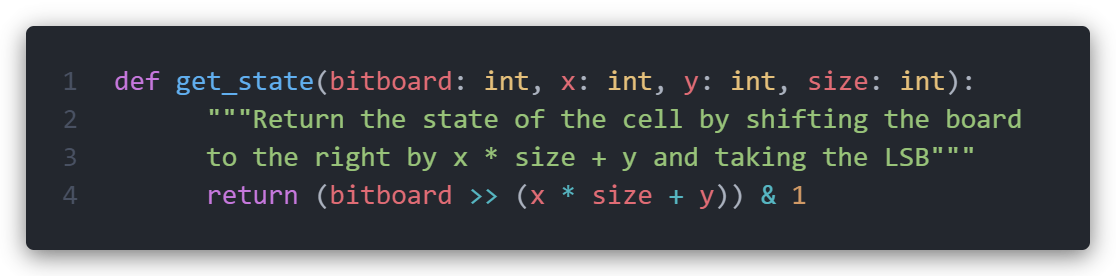
\includegraphics[width=1\textwidth]{ressources/get_state.png}
    \caption{Opérations logiques pour obtenir l'état du plateau.}
    \label{fig:get_state}
\end{figure}
\begin{figure}[H]
    \centering
    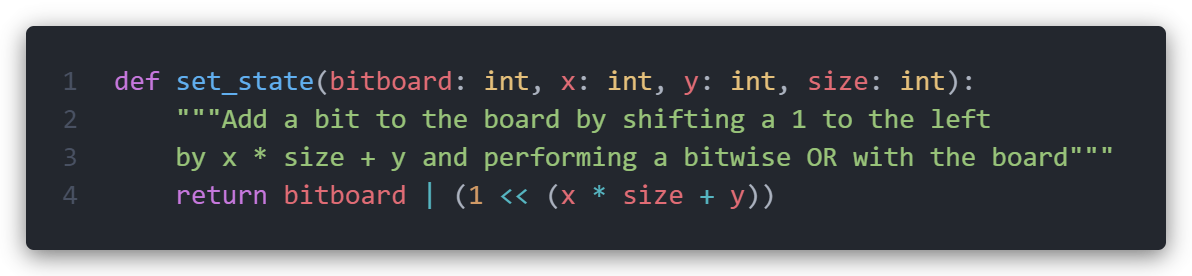
\includegraphics[width=1\textwidth]{ressources/set_state.png}
    \caption{Opérations logiques pour définir l'état du plateau.}
    \label{fig:set_state}
\end{figure}

En \ref{subsec:shift}, nous avons vu comment décaler un bitboard dans 4 directions cardinales. Voyons maintenant comment décaler un bitboard dans les 4 directions diagonales, et leur équivalent en python.

\begin{algorithm}[H]
    \caption{Opérations de décalage en diagonales.}
    \begin{algorithmic}[1]
    \Function{NordEst}{$x$}
        \State \Return $Nord(Est(x))$
    \EndFunction

    \Function{NordOuest}{$x$}
        \State \Return $Nord(Ouest(x))$
    \EndFunction

    \Function{SudEst}{$x$}
        \State \Return $Sud(Est(x))$
    \EndFunction

    \Function{SudOuest}{$x$}
        \State \Return $Sud(Ouest(x))$
    \EndFunction
    \end{algorithmic}
\end{algorithm}

\noindent \textbf{En Python :}
\begin{figure}[H]
    \centering
    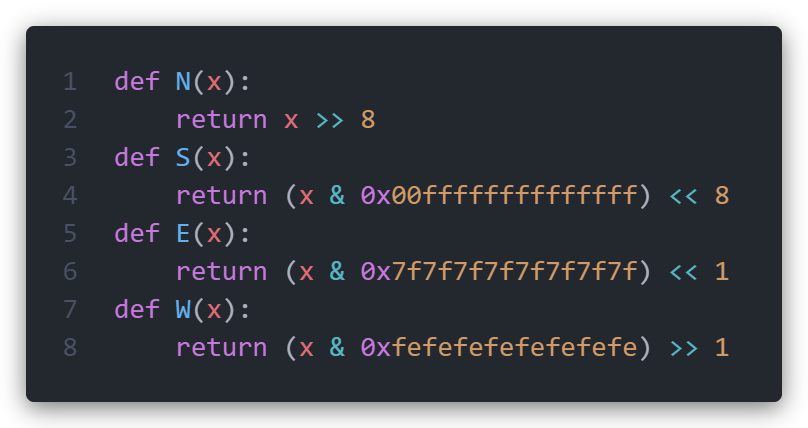
\includegraphics[width=0.8\textwidth]{ressources/operateurCardinaux.png}
    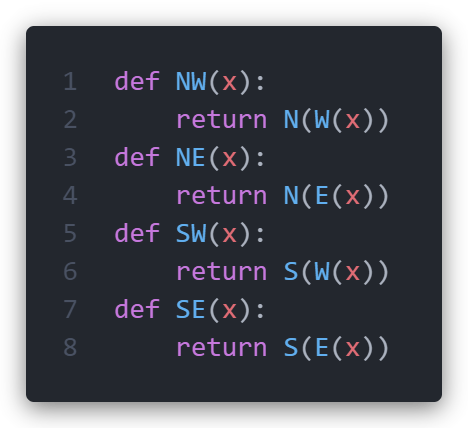
\includegraphics[width=0.5\textwidth]{ressources/operateurCardinauxComposes.png}
    \caption{Opérations de décalage pour les coups valides.}
    \label{fig:shift_ops}
\end{figure}

\section{Trouver et jouer coups valides}
\label{app:valid_moves}

En \ref{subsec:valid_moves}, nous avons vu comment trouver les coups valides et les jouer. Voyons maintenant en Python comment se traduit les pseudo-codes.

\begin{figure}[H]
    \centering
    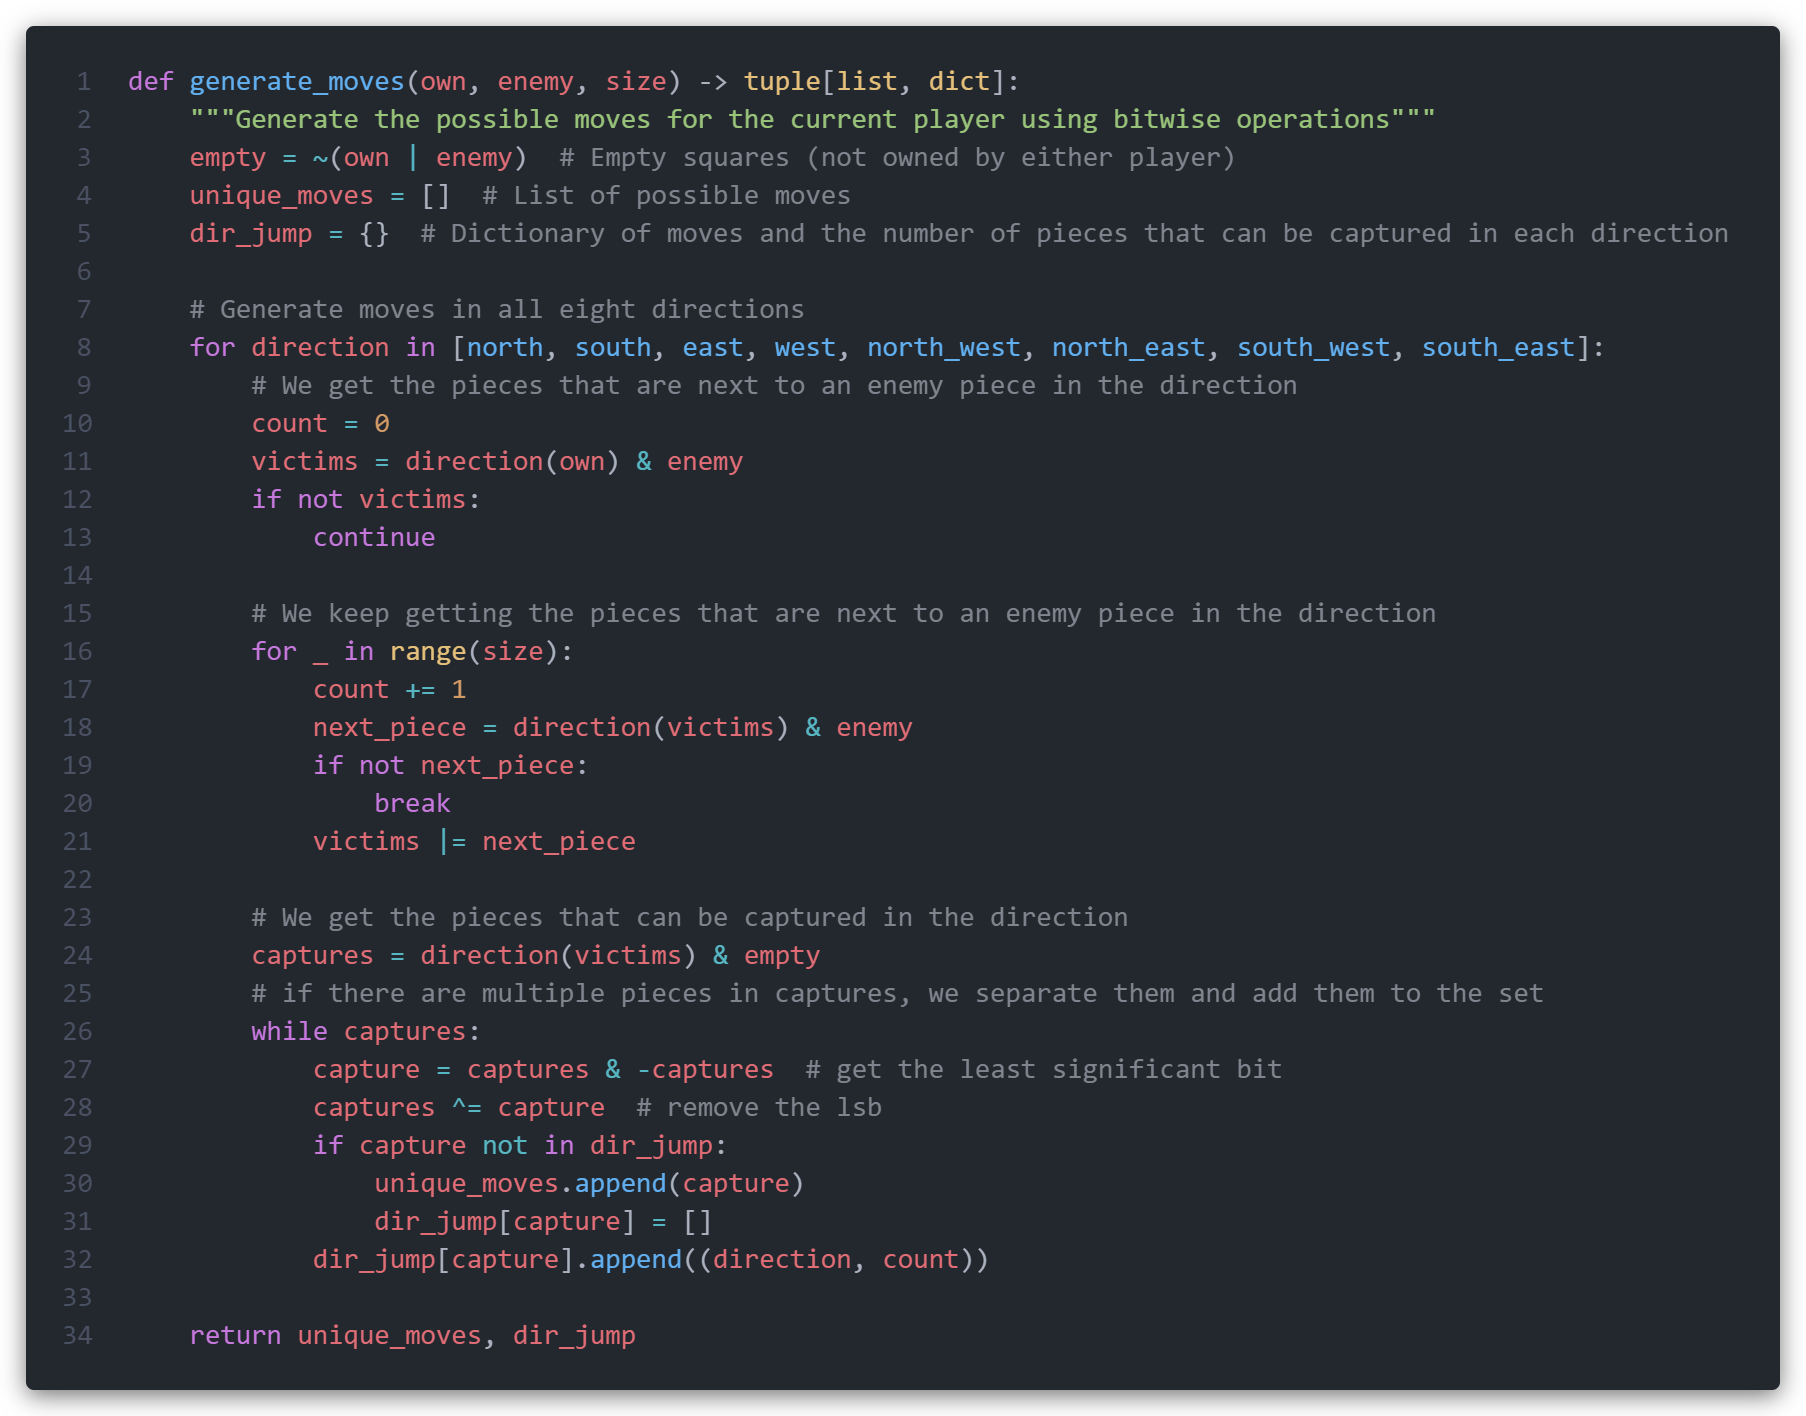
\includegraphics[width=1\textwidth]{ressources/generate_moves.png}
    \caption{Trouver les coups valides.}
    \label{fig:generate_moves}
\end{figure}

\begin{figure}[H]
    \centering
    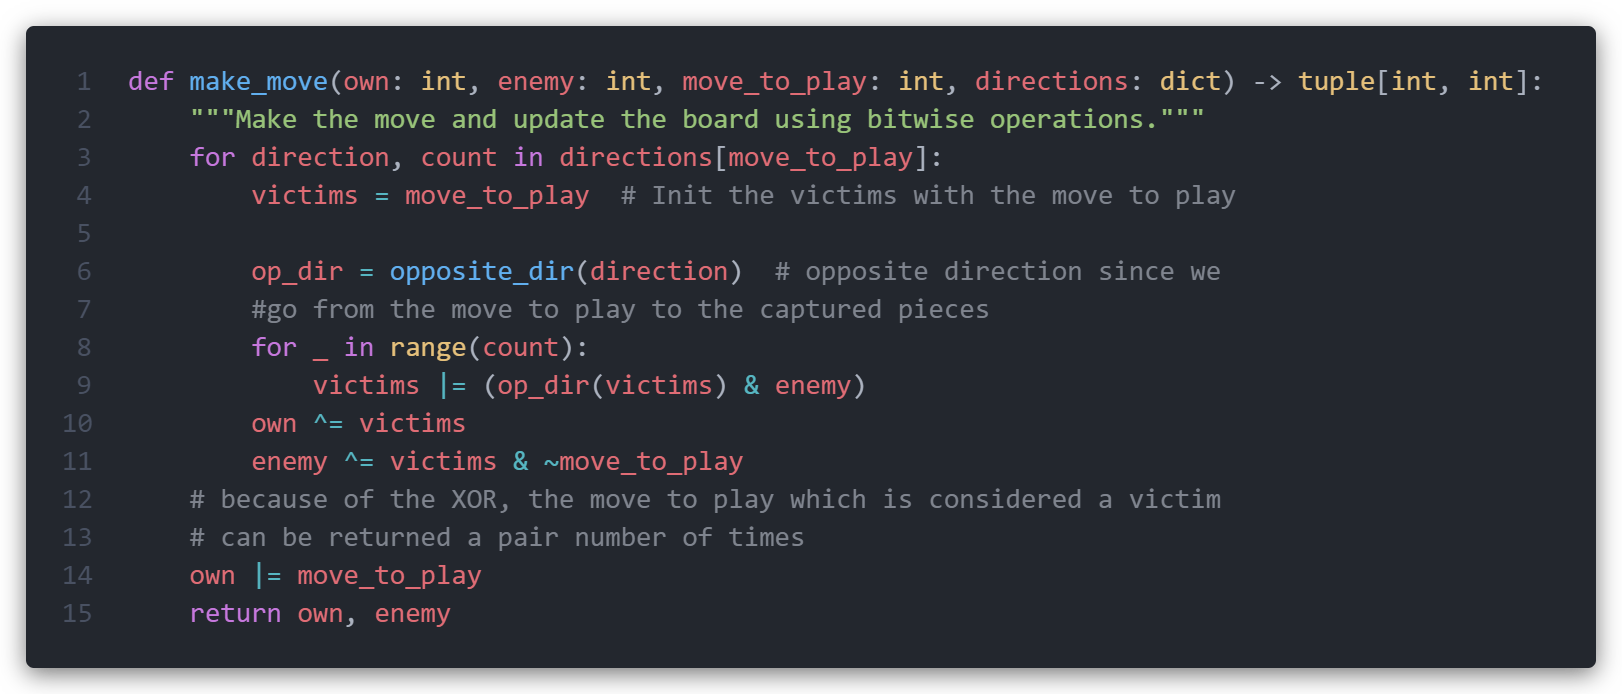
\includegraphics[width=1\textwidth]{ressources/make_move.png}
    \caption{Jouer un coup.}
    \label{fig:make_move}
\end{figure}

\section{Minimax}
\label{app:minimax}

En \ref{subsec:minimax}, nous avons vu comment implémenter l'algorithme Negamax avec AlphaBeta. Voyons maintenant en Python comment se traduit le pseudo-code, et les autres versions de l'algorithme.

\begin{figure}[H]
    \centering
    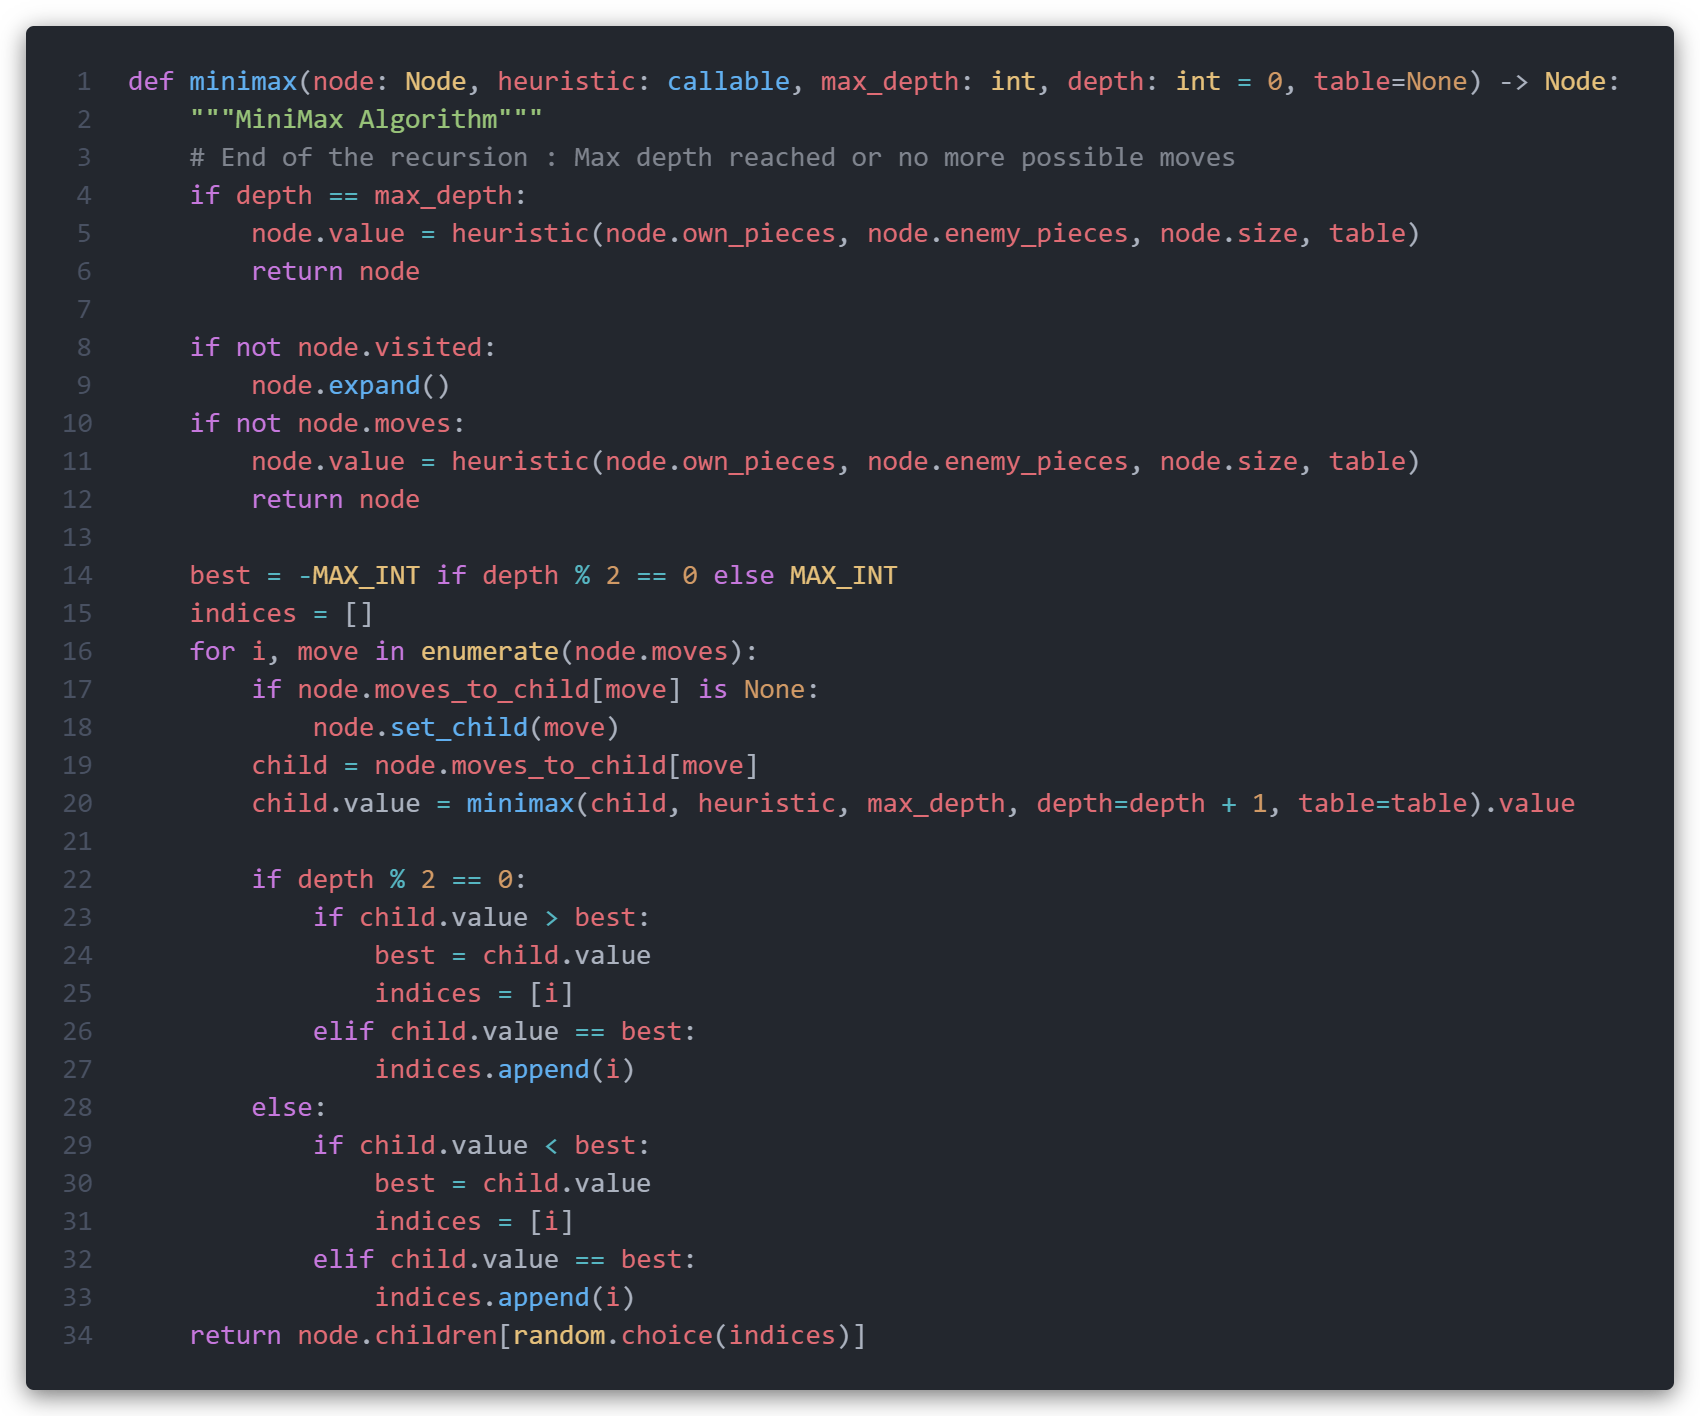
\includegraphics[width=1\textwidth]{ressources/minimax.png}
    \caption{Algorithme Minimax.}
    \label{fig:minimax}
\end{figure}

\begin{figure}[H]
    \centering
    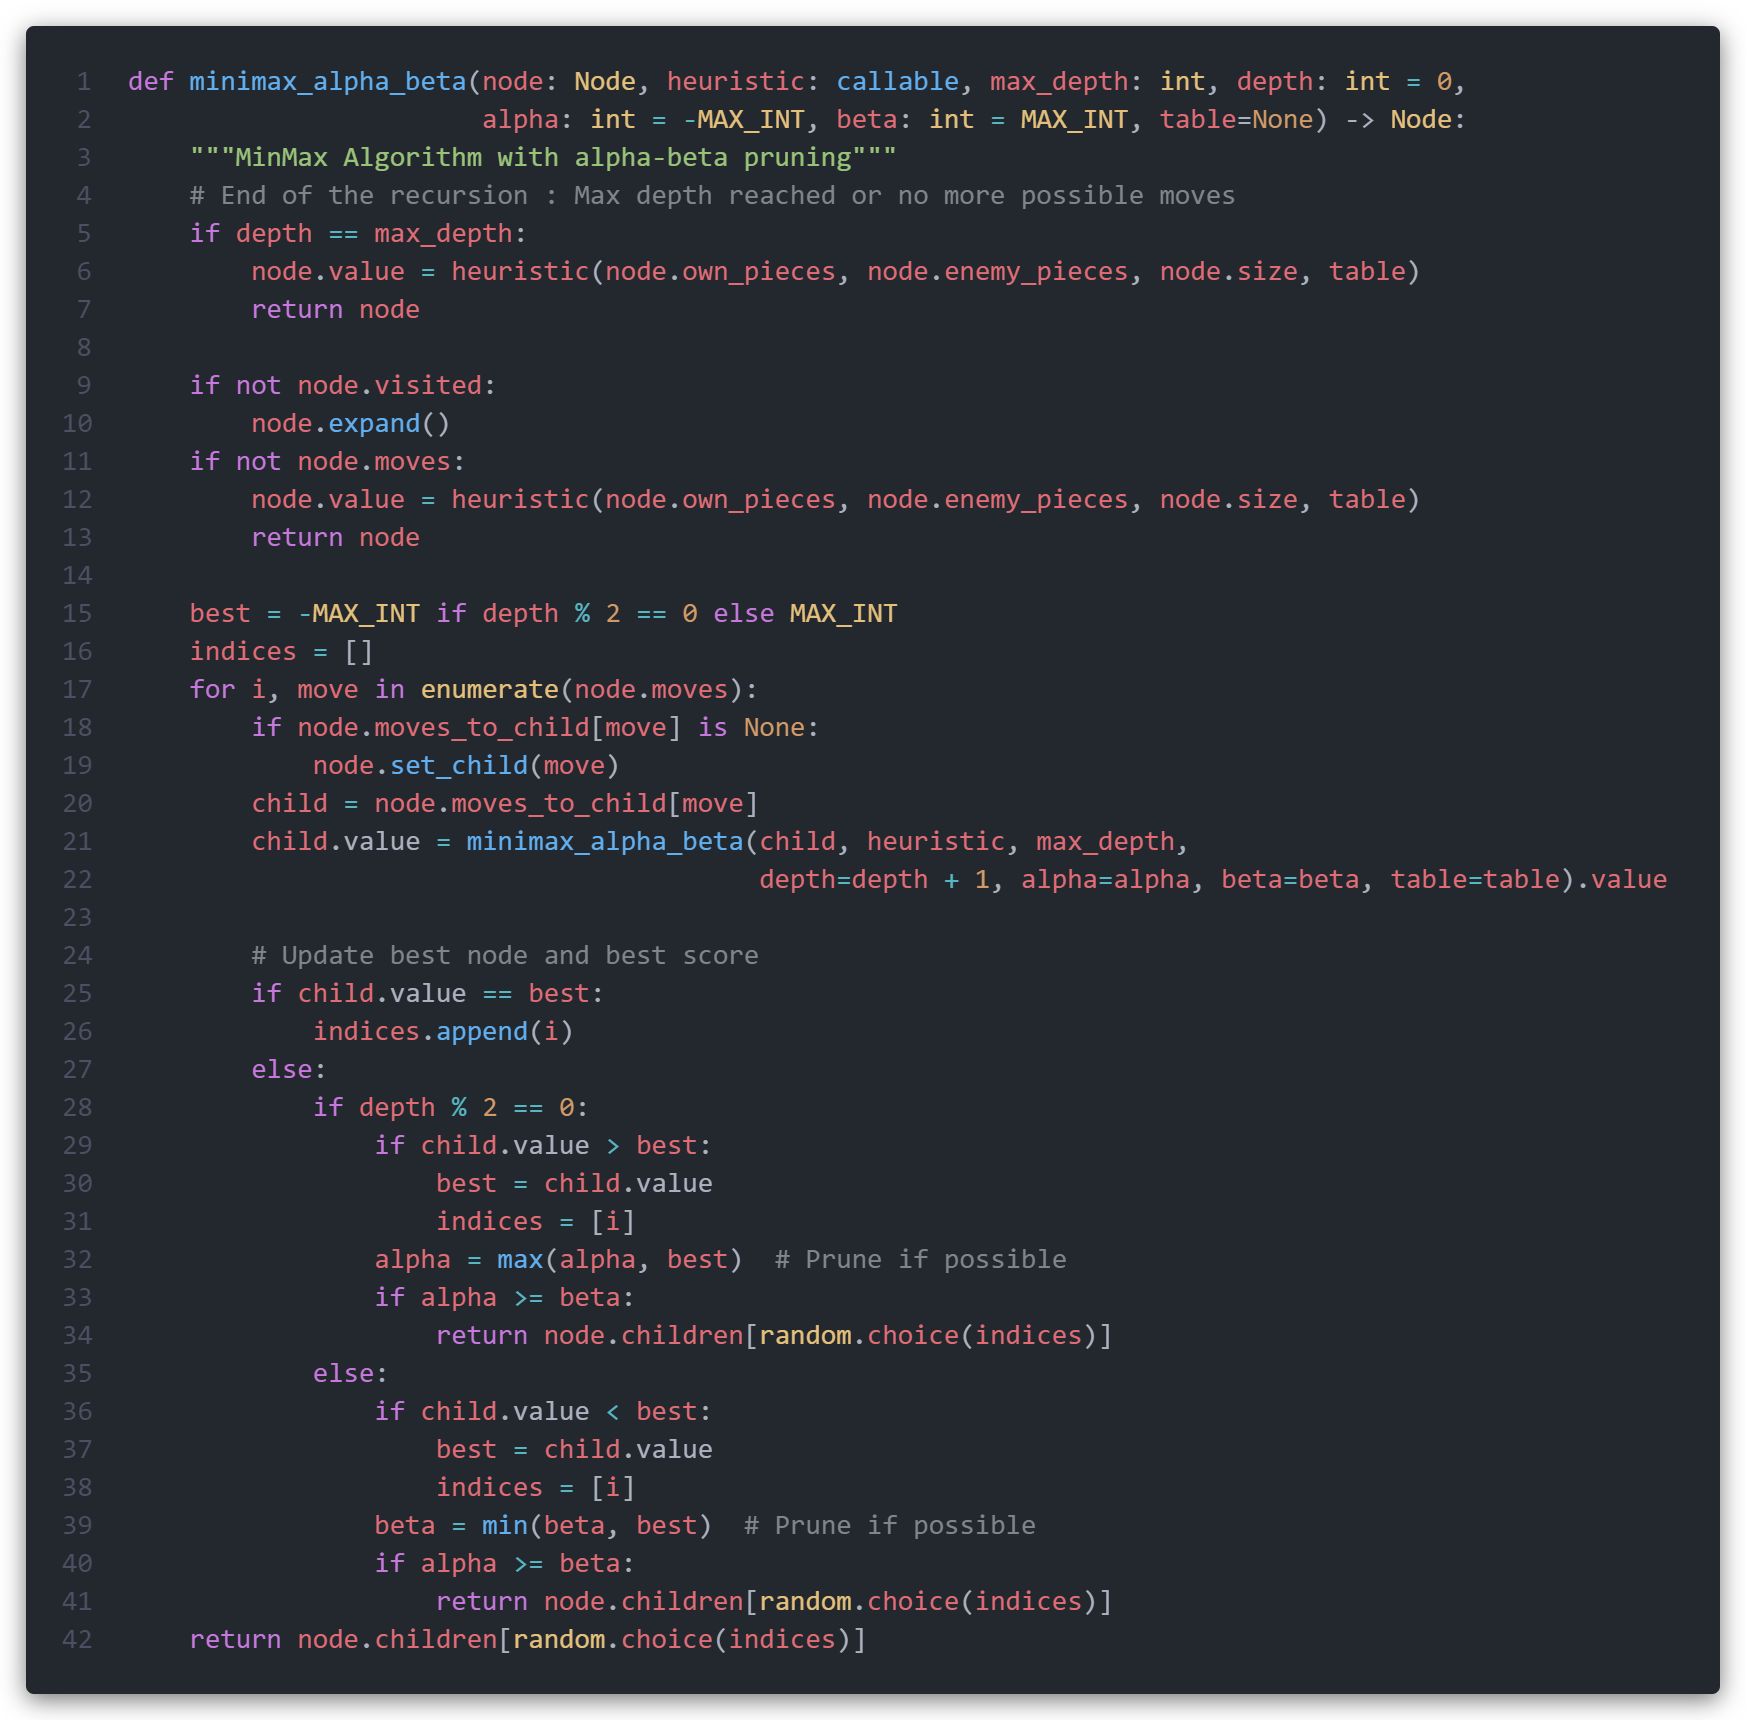
\includegraphics[width=1\textwidth]{ressources/minimax-a-b.png}
    \caption{Algorithme Minimax avec AlphaBeta.}
    \label{fig:minimax-a-b}
\end{figure}

\begin{figure}[H]
    \centering
    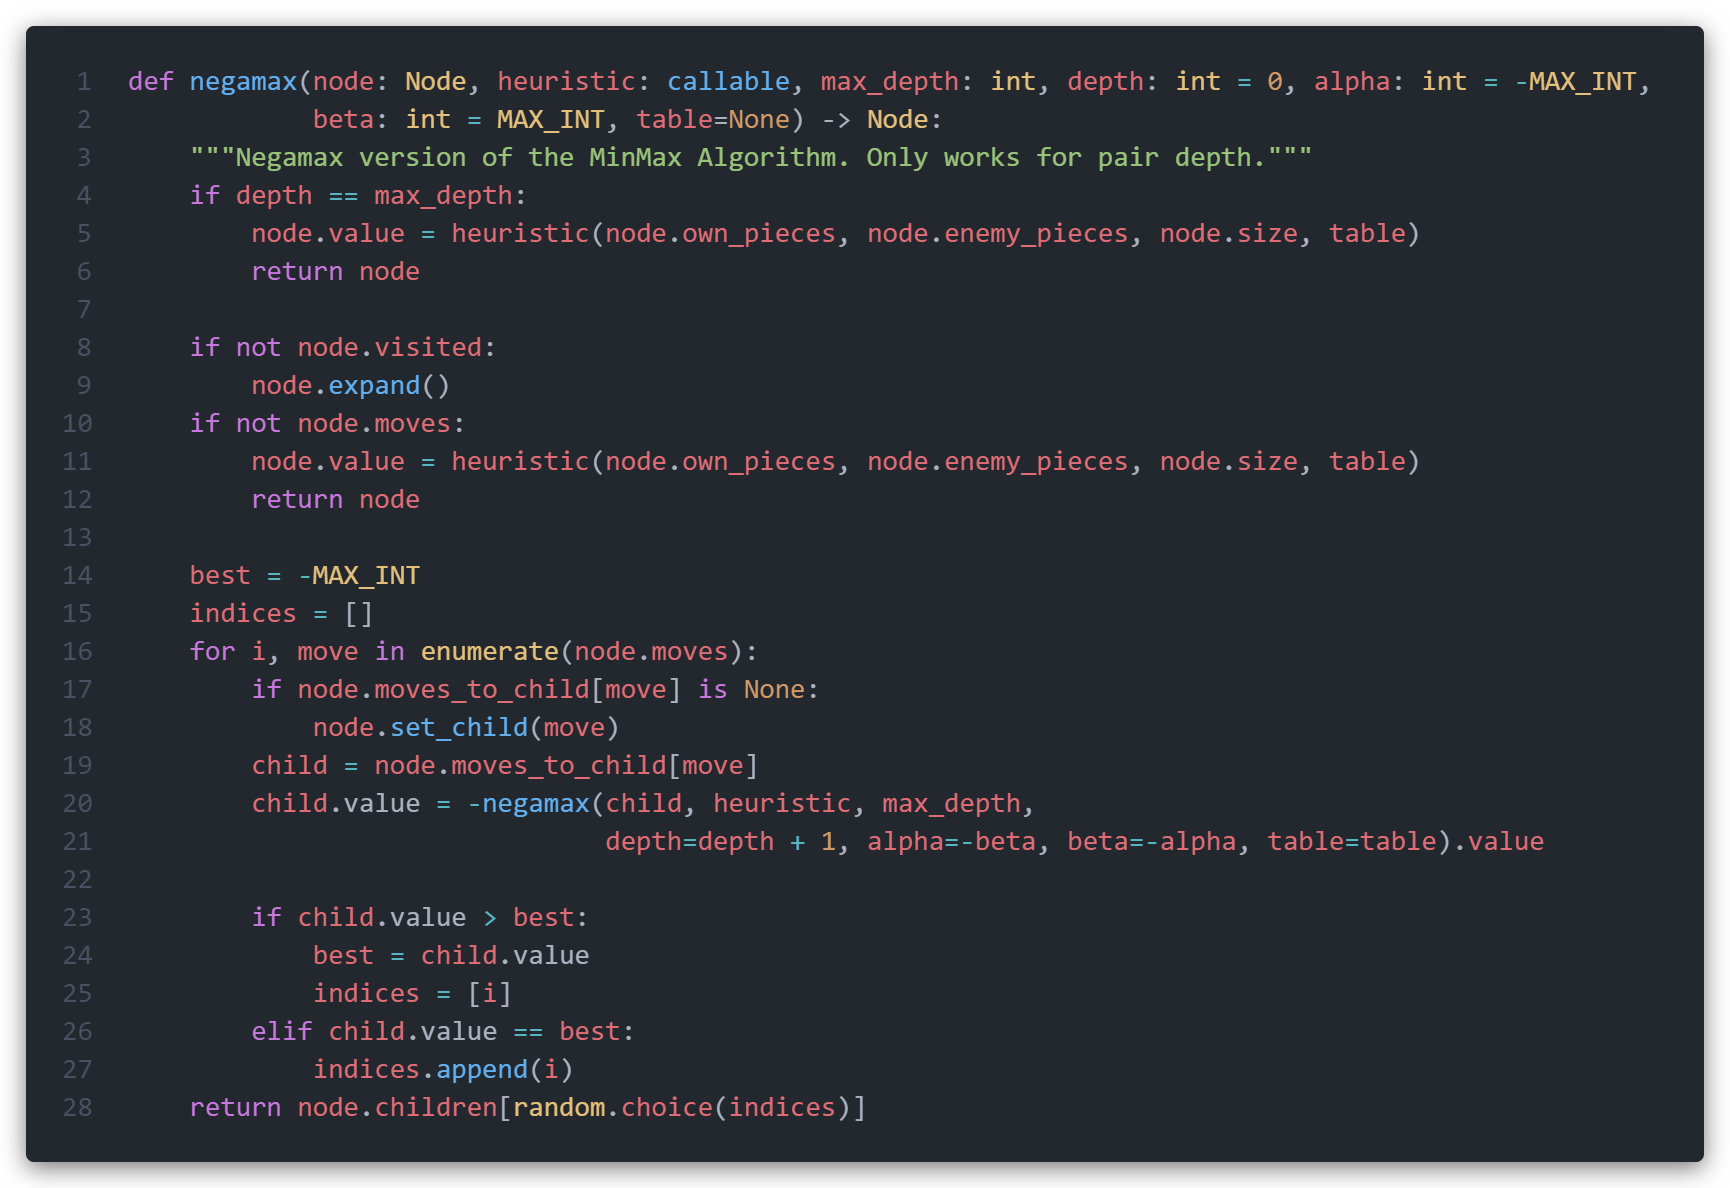
\includegraphics[width=1\textwidth]{ressources/negamax.png}
    \caption{Algorithme Negamax.}
    \label{fig:negamax}
\end{figure}


\begin{figure}[H]
    \centering
    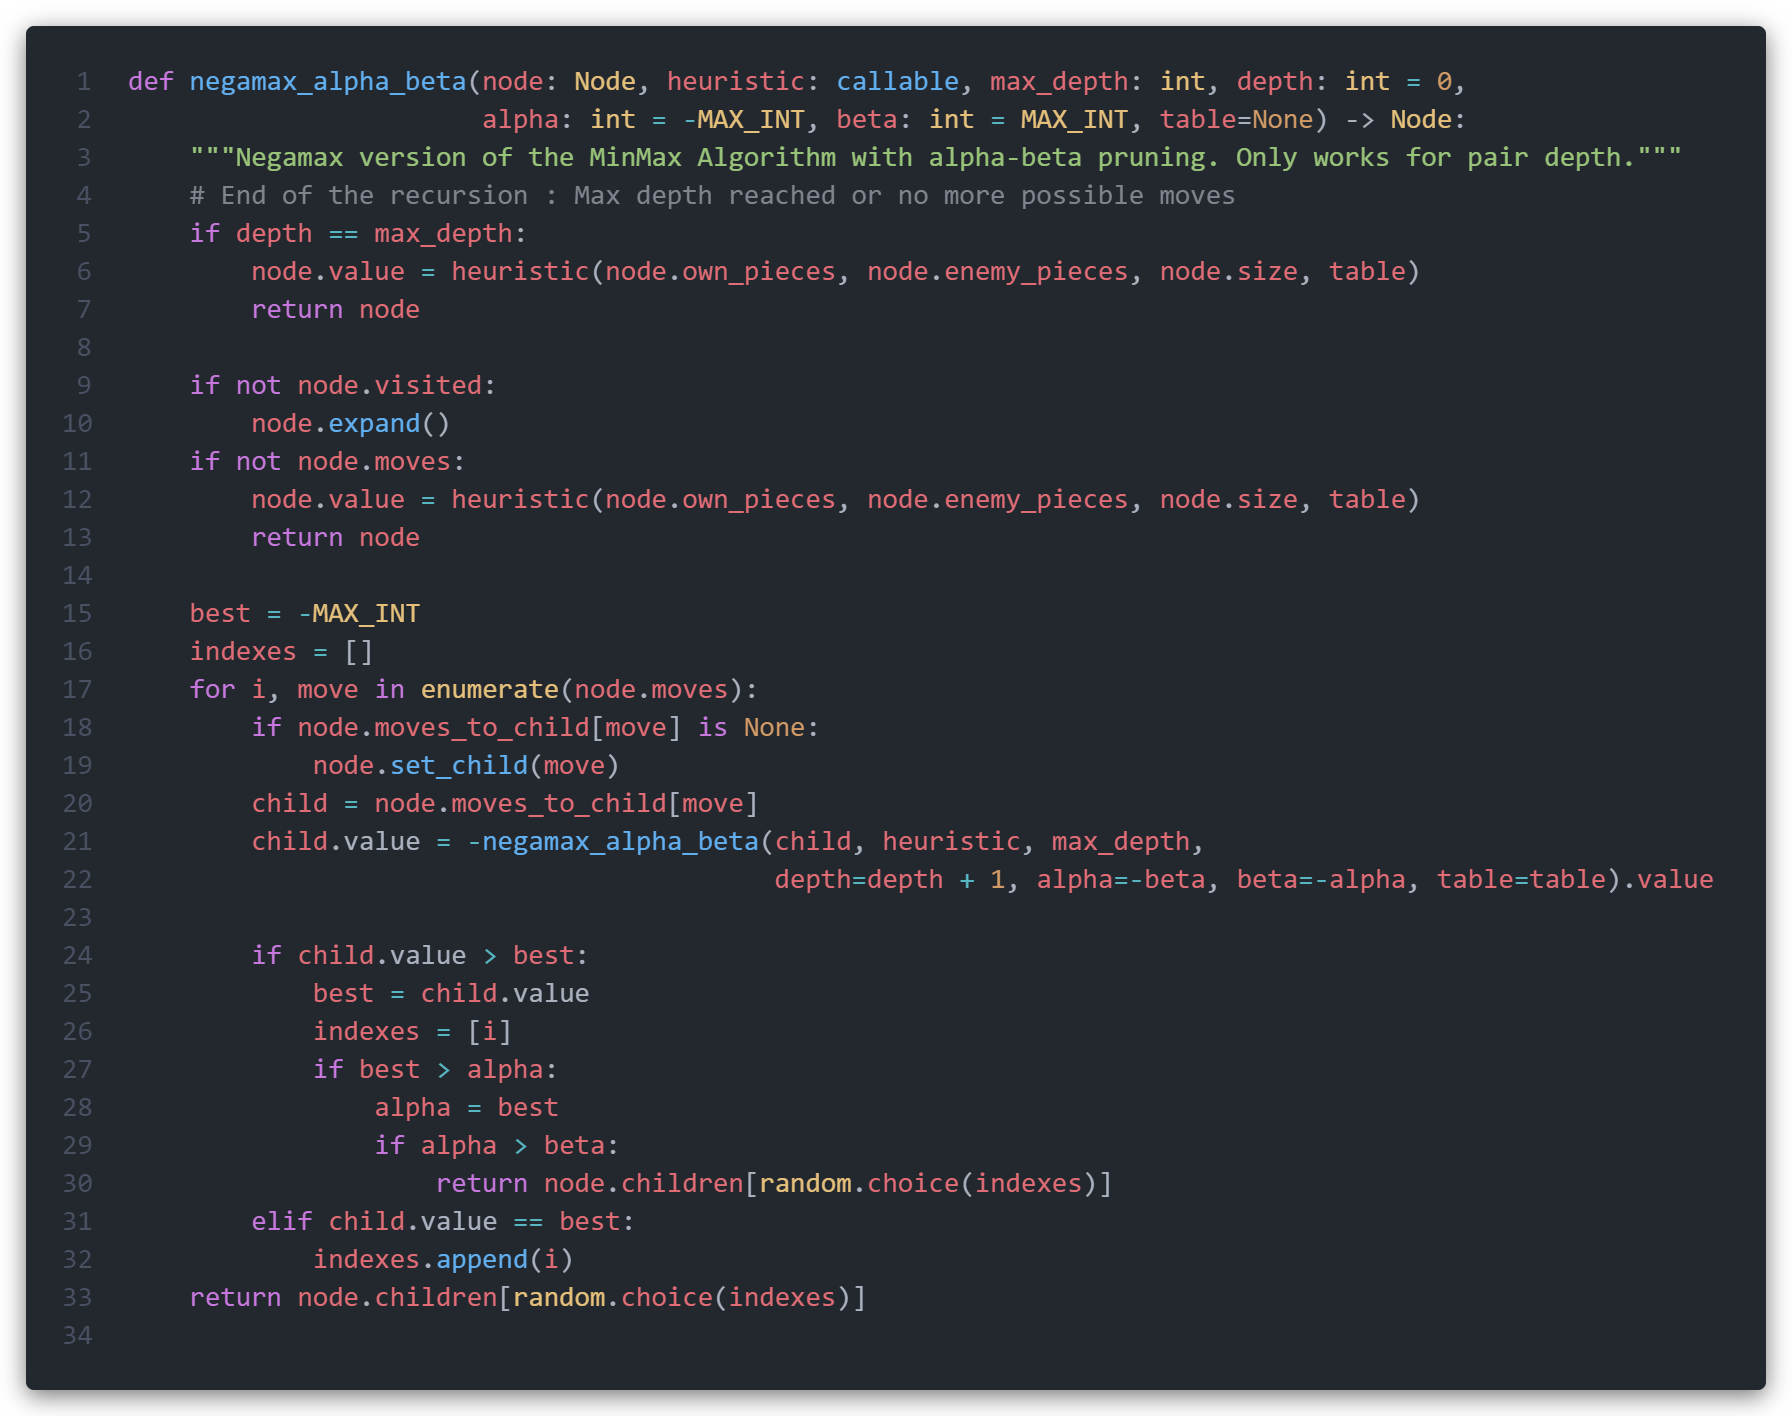
\includegraphics[width=1\textwidth]{ressources/nega-a-b.png}
    \caption{Algorithme Negamax avec AlphaBeta.}
    \label{fig:negamax-a-b}
\end{figure}